%=====================================================================
% Advanced Fiber Materials / Springer Nature LaTeX Manuscript
%=====================================================================

\documentclass[pdflatex,sn-mathphys-num,iicol]{sn-jnl}

%=====================================================================
% Packages
%=====================================================================
\usepackage{graphicx}
\usepackage{multirow}
\usepackage{amsmath,amssymb,amsfonts}
\usepackage{amsthm}
\usepackage{mathrsfs}
\usepackage[title]{appendix}
\usepackage{xcolor}
\usepackage{textcomp}
\usepackage{manyfoot}
\usepackage{booktabs}
\usepackage{algorithm}
\usepackage{algorithmicx}
\usepackage{algpseudocode}
\usepackage{listings}
\usepackage{url}

%=====================================================================
% Code listing settings
%=====================================================================
\lstset{
basicstyle=\small\ttfamily,
breaklines=true,
frame=single,
columns=fullflexible,
captionpos=b
}

%=====================================================================
% Theorem settings
%=====================================================================
\theoremstyle{thmstyleone}
\newtheorem{theorem}{Theorem}

\theoremstyle{thmstyletwo}
\newtheorem{example}{Example}
\newtheorem{remark}{Remark}

\theoremstyle{thmstylethree}
\newtheorem{definition}{Definition}

\raggedbottom

\begin{document}

%=====================================================================
% TITLE
%=====================================================================

\title[SEM Defect Quantification for Fiber-Related Perovskite Photovoltaics]
{Interpretable SEM-Based Microdefect Quantification for Fiber-Related
and Flexible Perovskite Photovoltaic Materials}

%=====================================================================
% AUTHORS
%=====================================================================

\author*[1]{\fnm{Sahil} \sur{Soni}}\email{your-email@example.com}

\affil*[1]{
\orgdiv{Department of Artificial Intelligence and Machine Learning},
\orgname{Symbiosis Institute of Technology, Symbiosis International (Deemed University)},
\orgaddress{\city{Pune}, \state{Maharashtra}, \country{India}}
}

%=====================================================================
% ABSTRACT
%=====================================================================

\abstract{
Fiber-related and flexible perovskite photovoltaic materials are
promising for lightweight, wearable, and green-energy harvesting
applications, but their device reliability depends strongly on
thin-film morphology. Microstructural defects such as pinholes, voids,
incomplete coverage, and non-uniform grains can create leakage
pathways, enhance charge recombination, reduce effective
light-absorbing area, and accelerate instability. Recent experimental
studies have shown that nanovoids of approximately 100--200~nm
diameter, directly observable in scanning electron microscopy (SEM)
images, are associated with increased trap-state density and
measurably reduced fill factor and power conversion efficiency in
wide-bandgap perovskite devices. Eliminating such voids through
process optimisation has been shown to improve certified efficiency
from approximately 22\% to over 23\% in state-of-the-art inverted
devices. Manual SEM inspection, however, is slow, subjective, and
difficult to scale for fabrication quality control. This study
presents an interpretable computer-vision pipeline for SEM-based
microdefect quantification in perovskite photovoltaic films, with
emphasis on fiber-related and flexible device inspection. The proposed
method combines grayscale preprocessing, contrast-limited adaptive
histogram equalization, dynamic thresholding based on image intensity
statistics, morphological refinement, and contour-based defect
filtering. Unlike fixed-threshold segmentation, the method adapts to
variations in SEM contrast, illumination, and local texture. The
pipeline is evaluated against manual annotation and classical
baselines, including Otsu thresholding, contrast-enhanced Otsu
thresholding, Canny edge detection, and watershed segmentation. The
output includes defect masks, defect count, total defect area, mean
defect diameter, and defect-area percentage, enabling direct
connection between image features and material-quality indicators
relevant to photovoltaic device performance. This work provides a
lightweight and reproducible route for scalable SEM morphology
analysis in perovskite photovoltaic material development.
}

%=====================================================================
% KEYWORDS
%=====================================================================

\keywords{
Perovskite photovoltaics, SEM morphology, fiber-related solar cells,
flexible solar cells, microdefect quantification, green-energy materials
}

\maketitle

%=====================================================================
% 1. INTRODUCTION
%=====================================================================

\section{Introduction}\label{sec:introduction}

Perovskite photovoltaic materials have attracted strong attention for
next-generation solar-energy conversion because of their high optical
absorption, tunable band gap, solution-processability, and
compatibility with lightweight and flexible device architectures
\cite{kojima2009,snaith2013,green2014,park2015}.
Recent progress has been remarkable: inverted perovskite solar cells
have reached certified efficiencies exceeding 27\% for narrow-bandgap
compositions \cite{green2025}, while wide-bandgap (1.65--1.80~eV)
inverted devices have surpassed 23\% certified efficiency with fill
factors as high as 86.8\% \cite{chang2026}. High-efficiency
perovskite/silicon tandem and triple-junction configurations have
reached 30.97\% and 27.06\% respectively
\cite{chang2026,zheng2025}, making perovskite photovoltaics a
central technology in high-performance solar-energy conversion.

Beyond conventional planar devices, flexible and fiber-related
perovskite solar cells are increasingly important for wearable
electronics, smart textiles, curved surfaces, portable power systems,
and distributed green-energy harvesting
\cite{balilonda2019,hu2016,qiu2016,diGiacomo2016}.
In such non-planar and mechanically adaptable configurations, film
uniformity becomes especially critical because bending, coating on
curved substrates, and scalable deposition can increase the
probability of local microstructural defects. As devices approach
the Shockley--Queisser limit, the dominant performance bottleneck
shifts from bulk recombination to interfacial and morphological
defects, making their systematic quantification increasingly
important.

Microstructural defects such as pinholes, voids, incomplete coverage,
rough grains, and non-uniform crystallisation can strongly influence
photovoltaic performance. Recent experimental evidence directly
confirms these connections. Chang et al.\ \cite{chang2026} reported
that perovskite films deposited on single-component hole-transport
layers exhibit nanovoids with an average diameter of
$144.6 \pm 56.9$~nm, as observed in SEM images. These voids were
found to facilitate non-radiative recombination and hinder efficient
charge-carrier transport, contributing to a trap-state density of
$2.62 \times 10^{16}$~cm$^{-3}$ at the buried interface. When the
hole-transport layer was optimised to eliminate such voids, the
trap-state density was reduced by 14.8\% and the power conversion
efficiency improved from 21.92\% to 23.04\% for 1.67~eV wide-bandgap
devices, with a certified fill factor of 86.8\% \cite{chang2026}.
Similarly, Zheng et al.\ \cite{zheng2025} used cross-sectional SEM
imaging to confirm the absence of voids and delamination in
high-performance triple-junction cells achieving 27.06\% certified
efficiency, validating SEM morphology analysis as a standard
quality-control tool in state-of-the-art photovoltaic research.

Pinholes may expose the underlying charge-transport layer, form local
shunting paths, and reduce the effective light-absorbing area.
Void-like regions can interrupt film continuity and create local
current-collection losses. The formation of voids has been attributed
to the trapping and subsequent escape of the high-boiling-point
solvent DMSO during film deposition \cite{chang2026,chen2021}.
Non-uniform grain morphology and high-defect-density regions increase
non-radiative recombination and accelerate degradation under moisture,
heat, light, and mechanical stress. Therefore, microdefect inspection
is not only an image-processing task but also a
materials-characterisation problem connected to device efficiency,
stability, reproducibility, and manufacturing yield.

Scanning electron microscopy (SEM) is widely used to examine
perovskite thin-film morphology because it provides high-resolution
surface information. SEM images allow researchers to visually inspect
pinhole formation, grain structure, local cracks, incomplete surface
coverage, and coating defects. As demonstrated across recent
high-impact studies \cite{chang2026,zheng2025}, SEM morphology
assessment is a standard step in verifying film quality before and
after process optimisation. However, manual SEM inspection is slow,
subjective, and difficult to reproduce across large fabrication
batches. This limitation is more serious for flexible and
fiber-integrated devices, where film morphology may vary along curved
or elongated geometries. For scalable green-energy manufacturing,
there is a need for automated and interpretable tools that can convert
SEM morphology into quantitative defect indicators.

Traditional computer-vision methods such as global thresholding,
Otsu thresholding, edge detection, and watershed segmentation are
commonly used for image segmentation
\cite{otsu1979,canny1986,vincent1991}. These techniques are simple
and computationally efficient, but their performance may degrade when
SEM images contain uneven illumination, low contrast, charging
artefacts, or complex nanoscale texture. Deep learning approaches
can improve detection accuracy but require carefully annotated
datasets and high computational resources. For early-stage materials
research with limited annotations, interpretable computer-vision
pipelines remain valuable.

This study proposes an interpretable SEM-based microdefect
quantification pipeline for perovskite photovoltaic materials, with
emphasis on fiber-related and flexible device inspection. The pipeline
combines contrast-limited adaptive histogram equalization (CLAHE),
dynamic thresholding, morphological refinement, and contour-based
filtering to identify pinhole-like and void-like regions of the type
documented in recent high-performance perovskite device studies
\cite{chang2026,zheng2025}.

The main contributions of this work are:

\begin{itemize}
\item A materials-aware SEM analysis pipeline is proposed for
microdefect quantification in perovskite photovoltaic films,
targeting morphological features directly linked to device
performance loss.
\item The work is framed for fiber-related and flexible perovskite
solar-cell inspection, where coating uniformity and scalable quality
control are critical.
\item Pinholes and voids are treated as material-quality indicators
linked to film coverage, leakage pathways, non-radiative
recombination, and stability, consistent with findings reported in
state-of-the-art perovskite device literature \cite{chang2026,hu2023}.
\item Dynamic thresholding and CLAHE are integrated to improve
robustness under SEM contrast and illumination variation.
\item The proposed method is validated against manual annotation and
classical segmentation baselines including Otsu, CLAHE+Otsu, Canny,
and watershed.
\item The method outputs defect masks and measurable descriptors such
as defect count, total defect area, mean defect diameter, and
defect-area percentage, which can be compared across fabrication
conditions and device batches.
\end{itemize}

%=====================================================================
% 2. MATERIALS RELEVANCE AND SEM MORPHOLOGY MOTIVATION
%=====================================================================

\section{Materials Relevance and SEM Morphology Motivation}
\label{sec:materials_relevance}

\subsection{Microdefects in Perovskite Photovoltaic Films}
\label{subsec:microdefects}

In perovskite photovoltaic films, microdefects are closely related to
film formation, crystallisation, solvent evaporation, substrate
wetting, and post-treatment conditions. A visually small defect in an
SEM image may correspond to incomplete perovskite coverage, a local
void, or a weakly connected grain region. Such defects can disturb
charge transport and reduce the spatial uniformity of photocurrent
generation.

Recent experimental evidence provides quantitative context for this
connection. Chang et al.\ \cite{chang2026} reported that SEM images
of wide-bandgap ($\sim$1.67~eV) formamidinium-based perovskite films
deposited on single-component hole-transport layers revealed nanovoids
with an average diameter of $144.6 \pm 56.9$~nm. These voids were
attributed to the segregation of the high-boiling-point solvent DMSO,
which becomes trapped within the perovskite film during deposition and
escapes from the bottom, leaving voids behind
\cite{chang2026,chen2021}. This mechanism is especially relevant
during multi-step spin-coating processes used in both planar and
flexible device fabrication.

When such voids were eliminated through hole-transport layer
engineering, the device power conversion efficiency improved from
21.92\% to 23.04\%, accompanied by improvements in V$_{oc}$, FF,
and J$_{sc}$ \cite{chang2026}. The fill factor reached a certified
value of 86.8\% in the void-free configuration. This demonstrates
that even nanoscale voids visible in SEM images carry measurable
consequences for macroscopic device performance.

Pinholes and voids are particularly important because they can form
electrical leakage channels between the electron- and hole-transport
layers. In a solar cell, this may increase shunt pathways and reduce
open-circuit voltage or fill factor. In flexible and fiber-shaped
perovskite devices, such defects may become more severe because the
active layer is deposited on curved, rough, or mechanically
deformable surfaces. Hence, automated pinhole and void quantification
can support process optimisation for coating uniformity and device
reproducibility.

\subsection{Physical Mechanisms Linking SEM Morphology to Device Performance}
\label{subsec:physical_mechanisms}

Understanding the physical origin of SEM-visible defects is essential
for interpreting automated quantification results as materials-quality
indicators. The following mechanisms connect SEM-observable
morphology to device physics.

\textbf{Void formation and solvent trapping.}
DMSO, commonly used with DMF to dissolve perovskite precursors, tends
to become trapped within the film during spin-coating and escapes from
the bottom during annealing, leaving voids behind
\cite{chang2026,chen2021}. These voids appear as dark regions in
top-view SEM images, making them detectable by intensity-based
segmentation.

\textbf{Non-radiative recombination and trap-state density.}
Trap-state densities at the perovskite/hole-transport-layer interface
have been measured by space-charge-limited current analysis. A
trap-state density of $2.62 \times 10^{16}$~cm$^{-3}$ was reported
for void-containing films, reduced by 14.8\% to
$2.24 \times 10^{16}$~cm$^{-3}$ when voids were eliminated
\cite{chang2026}. This quantitative link between SEM-observable
morphology and trap density is the physical justification for
treating the pipeline output as a materials-quality indicator.

\textbf{Phase segregation and illumination stability.}
Perovskite films with higher void coverage show more pronounced
photo-induced halide segregation under continuous illumination,
as monitored by time-resolved photoluminescence \cite{chang2026}.
Charge accumulation at defect-rich regions promotes ion migration
and bandgap redshift, which reduces long-term photovoltaic stability.

\textbf{Interface quality in multi-junction architectures.}
For tandem and triple-junction devices, cross-sectional SEM imaging
is used to confirm layer continuity and absence of voids at buried
interfaces \cite{zheng2025}. In a triple-junction
perovskite/perovskite/silicon device achieving 27.06\% certified
efficiency, cross-sectional SEM confirmed continuous layers without
voids at each subcell interface \cite{zheng2025}. This illustrates
that SEM morphology verification is standard practice even in the
most advanced photovoltaic architectures.

\subsection{Relevance to Fiber-Related and Flexible Photovoltaics}
\label{subsec:fiber_relevance}

Fiber-related and flexible perovskite photovoltaic devices require
uniform deposition over non-traditional geometries such as curved
fibers, flexible polymer substrates, yarn-like structures, or
textile-compatible surfaces. Compared with rigid planar substrates,
these geometries introduce additional challenges in coating thickness
control, surface wetting, mechanical strain, and interfacial adhesion
\cite{balilonda2019,hu2016,qiu2016,diGiacomo2016}.

The void and pinhole formation mechanisms identified for planar
devices are expected to be more pronounced in fiber-shaped and
flexible geometries, where substrate curvature affects solvent
evaporation dynamics and film crystallisation uniformity. The
DMSO-trapping mechanism that produces voids in flat-substrate films
\cite{chang2026} would be further modulated by local substrate
geometry and coating speed on a curved fiber surface. Furthermore,
the void diameter range identified in recent literature
($\sim$100--200~nm \cite{chang2026}) falls within the spatial
resolution range accessible to SEM imaging, making automated
SEM-based detection a practical approach for fiber and flexible
device quality assessment.

Although the SEM images analysed in this study are obtained from
planar or locally flat regions, the proposed quantification strategy
is directly relevant to flexible and fiber-related perovskite
photovoltaics because the same defect types---pinholes, voids, and
incomplete coverage---are critical during scalable coating and device
integration. The method can be extended to curved-fiber SEM images,
flexible substrate films, and roll-to-roll processed perovskite
layers.

\subsection{From Image Objects to Material-Quality Indicators}
\label{subsec:image_to_material}

The proposed method treats detected regions as material-quality
indicators rather than isolated image objects. Each detected defect
is converted into measurable descriptors such as area, equivalent
diameter, spatial density, and defect-area percentage. These values
can be compared across fabrication batches, coating recipes,
annealing temperatures, precursor concentrations, or substrate
treatments.

The average nanovoid diameter of $144.6 \pm 56.9$~nm reported by
Chang et al.\ \cite{chang2026} represents the type of quantitative
descriptor that the proposed pipeline aims to produce automatically
from SEM images, rather than through manual measurement. Such
automated extraction enables larger-scale morphology studies across
many samples and conditions, which is important for process
optimisation in green-energy manufacturing.

The central objective of this work is therefore to bridge SEM image
analysis with materials characterisation by converting visual
morphology into reproducible quantitative indicators. These
indicators are grounded in the physical mechanisms connecting
SEM-observable defects to photovoltaic device performance, as
established by recent experimental literature
\cite{chang2026,zheng2025,hu2023}.

%=====================================================================
% 3. RELATED WORK
%=====================================================================

\section{Related Work}\label{sec:related_work}

\subsection{Perovskite and Fiber-Related Photovoltaic Materials}
\label{subsec:psc_related_work}

Perovskite solar cells have progressed rapidly since their early
demonstration as visible-light sensitisers \cite{kojima2009}. Their
high absorption coefficient and compatibility with thin-film
processing make them attractive for flexible and lightweight
photovoltaic systems \cite{snaith2013,green2014,park2015}. Inverted
(p-i-n) device architectures now achieve certified efficiencies
exceeding 27\% for narrow-bandgap compositions \cite{green2025},
and wide-bandgap (1.67--1.73~eV) inverted devices have reached
certified efficiencies of 23.42\% with a fill factor of 86.8\%
\cite{chang2026}. These advances highlight the critical role of
interface quality, film morphology, and defect density in determining
photovoltaic performance.

At the system level, perovskite cells are increasingly integrated
into tandem and triple-junction architectures. A four-terminal
perovskite/silicon tandem achieved 30.97\% efficiency
\cite{chang2026}, while a monolithic perovskite/perovskite/silicon
triple junction reached a certified 27.06\% at 1~cm\textsuperscript{2}
and 23.3\% at 16~cm\textsuperscript{2} \cite{zheng2025}. These
state-of-the-art demonstrations routinely use SEM imaging for
morphological verification, confirming that SEM-based quality control
is a standard tool in high-performance photovoltaic research
\cite{chang2026,zheng2025}.

Fiber-shaped and flexible perovskite solar cells extend these
advantages toward wearable and textile-compatible energy harvesting,
but they also introduce additional challenges in morphology control,
coating uniformity, and mechanical durability
\cite{balilonda2019,hu2016,qiu2016,diGiacomo2016}.

\subsection{SEM Morphology and Defect-Performance Correlation}
\label{subsec:sem_morphology_correlation}

A growing body of experimental work directly links SEM-observable
morphological features to perovskite device performance. Chang et al.\
\cite{chang2026} demonstrated that nanovoids of average diameter
$144.6 \pm 56.9$~nm, observed in top-view SEM images of 1.67~eV
perovskite films, contributed to a trap-state density of
$2.62 \times 10^{16}$~cm$^{-3}$ and enhanced non-radiative
recombination at the buried interface. Eliminating these voids
reduced the trap-state density by 14.8\% and improved the certified
fill factor to 86.8\%.

Hu et al.\ \cite{hu2023} demonstrated a void-free buried interface
for scalable FAPbI\textsubscript{3} perovskite solar modules, showing
that void elimination at the buried interface directly improved module
stability and performance. Chen et al.\ \cite{chen2021} showed that
interfacial defects originating from void-related morphology
degradation were a primary cause of performance loss in perovskite
modules under operational conditions. In high-performance
triple-junction devices, cross-sectional SEM imaging confirmed
void-free and delamination-free interfaces as prerequisites for
achieving high fill factors \cite{zheng2025}.

These results collectively establish that SEM morphology analysis is
not a supplementary characterisation step but a primary method for
assessing perovskite film quality. However, all of the above studies
relied on manual SEM inspection. Automated and quantitative pipelines
that can extract defect descriptors from SEM images with
reproducibility and throughput remain an open need in the field.

\subsection{Computer Vision and Learning-Based Defect Detection}
\label{subsec:cv_related_work}

Classical segmentation methods such as Otsu thresholding, Canny edge
detection, and watershed segmentation are widely used because of
their simplicity and interpretability
\cite{otsu1979,canny1986,vincent1991}. CLAHE is useful for local
contrast enhancement and can improve defect visibility in
low-contrast images \cite{zuiderveld1994}. Deep learning methods such
as U-Net and YOLO have achieved strong performance in segmentation
and object detection tasks \cite{ronneberger2015,redmon2016}.
However, deep learning usually requires larger labelled datasets and
careful generalisation testing. For early-stage materials research
with limited annotations, interpretable computer-vision pipelines
remain valuable. Furthermore, the nanovoid diameter range observed
in perovskite SEM images ($\sim$100--200~nm \cite{chang2026}) is at
a spatial scale where intensity-based segmentation methods are
well-suited, provided sufficient contrast enhancement is applied
before thresholding.

%=====================================================================
% Literature Review Table
%=====================================================================

\begin{table*}[t]
\caption{Representative literature and research gap motivating the present study}
\label{tab:literature_review}
\begin{tabular}{@{}p{2.8cm}p{3.0cm}p{4.6cm}p{4.8cm}@{}}
\toprule
Reference & Area & Key contribution & Gap addressed in this work \\
\midrule
Kojima et al.\ \cite{kojima2009}
  & Perovskite photovoltaics
  & Demonstrated organometal halide perovskites for photovoltaic applications
  & Does not address automated morphology quantification \\[4pt]
Green et al.\ \cite{green2014}
  & Perovskite solar cells
  & Discussed emergence and rapid progress of perovskite solar cells
  & Focus is device progress rather than SEM defect analysis \\[4pt]
Chang et al.\ \cite{chang2026}
  & Wide-bandgap inverted PSC; tandem
  & SEM-visible nanovoids ($144.6 \pm 56.9$~nm) linked to 14.8\% higher
    trap density; void elimination improved certified PCE to 23.42\%
    with FF 86.8\%
  & Manual SEM used; no automated quantification pipeline \\[4pt]
Zheng et al.\ \cite{zheng2025}
  & Perovskite/perovskite/Si triple junction
  & SEM cross-sections verified void-free interfaces in 27.06\% cells;
    SEM used as standard quality gate
  & SEM used qualitatively; no defect descriptors extracted \\[4pt]
Balilonda et al.\ \cite{balilonda2019}
  & Perovskite solar fibers
  & Reviewed status and challenges of perovskite solar fibers
  & Highlights fiber relevance but not automated SEM quantification \\[4pt]
Hu et al.\ \cite{hu2016}
  & Fiber-shaped perovskite solar cells
  & Reported fiber-shaped perovskite solar-cell architecture
  & Does not provide automated microdefect detection workflow \\[4pt]
Otsu \cite{otsu1979}
  & Thresholding
  & Automatic threshold selection from gray-level histograms
  & Sensitive to SEM contrast and illumination variation \\[4pt]
Canny \cite{canny1986}
  & Edge detection
  & Widely used edge detector
  & Produces edges rather than material-defect regions \\[4pt]
Vincent and Soille \cite{vincent1991}
  & Watershed segmentation
  & Watershed segmentation for digital spaces
  & Can over-segment noisy SEM morphology \\[4pt]
Ronneberger et al.\ \cite{ronneberger2015}
  & Deep segmentation
  & U-Net for image segmentation
  & Requires annotated training data \\[4pt]
Present study
  & SEM defect quantification
  & Interpretable CV pipeline grounded in experimental perovskite literature
  & Defect masks, area fraction, mean defect diameter, baseline validation \\
\botrule
\end{tabular}
\end{table*}

%=====================================================================
% 4. MATERIALS AND DATASET
%=====================================================================

\section{Materials and Dataset}\label{sec:materials_dataset}

The experimental workflow consisted of perovskite film preparation,
structural and optical characterisation, SEM morphology imaging, and
automated defect quantification. The SEM images obtained from the
fabricated perovskite films were used as the primary input for the
proposed computer-vision pipeline.

\subsection{Chemicals and Materials}\label{subsec:chemicals_materials}

Dimethylformamide (DMF, 99.8\%), dimethyl sulfoxide (DMSO, 99.8\%),
ethyl acetate (anhydrous, 99.5\%), hexane (anhydrous, 99.5\%),
acetonitrile (99.8\%), ethanol (anhydrous, 99\%), and 2-propanol
(IPA, anhydrous, 99.9\%) were sourced from Sigma Aldrich. Lead(II)
iodide (PbI$_2$, 99.99\%) was obtained from Tokyo Chemical Industry.
Formamidinium iodide (FAI, $>$98\%), methylammonium bromide (MABr,
$>$98\%), phenethylammonium iodide (PEAI, $>$99\%), n-dodecylammonium
iodide (DDAI, $>$99\%), cyclohexylmethylammonium iodide (CMAI,
$>$99\%), 2-thiophenemethylammonium iodide (TMAI, $>$99\%), and
methylammonium chloride (MACl, $>$98\%) were procured from GreatCell
Solar and used as received \cite{ref23}.

\subsection{Fabrication of Perovskite Films}\label{subsec:fabrication}

ITO-coated or plain glass substrates were cleaned by sequential
sonication in acetone, ethanol, and 2-propanol, followed by 15~min
UV--ozone treatment. High-purity $\delta$-FAPbI$_3$ powder was
synthesised using a one-pot method \cite{ref23}. The powder was
washed three times with ethyl acetate and acetonitrile, dried in a
vacuum oven for more than 24~h, and stored in an N$_2$-filled
glovebox.

For pristine $\alpha$-FAPbI$_3$ films, a 1.8~M precursor solution
was prepared by dissolving 1139~mg $\delta$-FAPbI$_3$ and 40~mg
MACl in 1~mL DMF:DMSO (9:1 v/v). The solution was spin-coated on
the substrates in two steps: 1000~rpm for 10~s and 5000~rpm for 30~s.
During the second step, 100~$\mu$L of ethyl acetate:hexane (7:3 v/v)
antisolvent was applied at 10~s intervals under 30--40\% relative
humidity. The films were annealed at 150$^\circ$C for 20~min to form
$\alpha$-FAPbI$_3$. It should be noted that DMSO, used as part of
the precursor solvent system, has been identified as a key contributor
to void formation in perovskite films: DMSO tends to become trapped
within the film during deposition and escapes during annealing,
leaving voids behind \cite{chang2026,chen2021}. The presence and
size distribution of such voids in the final film were assessed using
SEM imaging and the automated pipeline described in this work.

For two-dimensional (2D) perovskite layers on three-dimensional (3D)
perovskite films, 4~mM solutions of PEAI, TMAI, CMAI, or DDAI in IPA
were sprayed at 3.0~mL/min using N$_2$ gas \cite{ref23}.

\subsection{Film Characterisation}\label{subsec:film_characterization}

Crystallographic properties were analysed using a Rigaku MiniFlex
X-ray diffractometer (XRD) with Cu K$\alpha$ radiation
($\lambda = 1.5405$~\AA). Absorption spectra were measured using a
Shimadzu UV-3600 Plus UV--vis--NIR spectrophotometer. Steady-state
photoluminescence (PL) was recorded using an Edinburgh Instruments
FS5 spectrofluorometer. Surface morphology was examined using a
JEOL/JSM-F100 scanning electron microscope.

The SEM images were used for morphology-based microdefect
quantification. Pinhole-like and void-like regions observed in SEM
images were treated as morphology indicators associated with
incomplete film coverage, local defect formation, and possible
leakage pathways in perovskite photovoltaic devices
\cite{chang2026,hu2023}. This interpretation is grounded in
experimental literature demonstrating direct correlation between
SEM-observable void density and trap-state density
\cite{chang2026}.

% TODO: Add exact SEM imaging details:
% - accelerating voltage
% - working distance
% - magnification range
% - image resolution (pixels)
% - scale bar value
% - number of SEM images in dataset
% - number of samples

\subsection{SEM Image Dataset for Defect Quantification}
\label{subsec:sem_dataset}

The SEM image dataset was constructed from morphology images obtained
during film characterisation and grouped into five defect and
morphology categories. In total, 440 SEM images were collected,
covering PbI$_2$ excess bright-particle regions, 3D perovskite
pinholes, 3D-2D mixed perovskite pinholes, 3D perovskite background
regions, and 3D-2D mixed perovskite background regions. For the YOLO
training and evaluation pipeline, these 440 base images were split
into 224$\times$224~pixel patches using a sliding-window strategy with
25\% overlap, producing 4{,}701 annotated patches distributed across
training (80\%), validation (10\%), and test (10\%) sets.
Table~\ref{tab:dataset_summary} summarises the dataset structure.

% TODO: Add exact SEM magnification, accelerating voltage, working
% distance, and image pixel resolution when available.

Manual annotations were prepared to provide a reference for validating
the automated segmentation results. Defect regions were marked based
on visual morphology, local darkness, boundary structure, and material
relevance. Very small isolated dark pixels were not considered defects
unless they satisfied the minimum area and shape criteria. The
expected void size range of $\sim$100--200~nm, as reported for similar
perovskite films in the literature \cite{chang2026}, was used as a
guide for setting the minimum area threshold $A_{min}$ in the pipeline.

\subsection{Defect Categories}\label{subsec:defect_categories}

The defect categories considered in this work include PbI$_2$ bright
particles, small pinholes, large pinholes, PbI$_2$ needle crystals,
and grain-boundary-associated defects. Pinholes and voids are defined
as local dark regions indicating incomplete film coverage. Bright
particles correspond to PbI$_2$ excess or undissolved crystallites
appearing as high-intensity spots. These regions are important because
they may contribute to charge leakage, non-radiative recombination,
reduced effective absorber coverage, and long-term instability in
perovskite photovoltaic devices \cite{chang2026,hu2023}.

\begin{table*}[t]
\caption{Summary of the SEM image dataset used for defect quantification
and YOLO model training}
\label{tab:dataset_summary}
\begin{tabular}{@{}lcccc@{}}
\toprule
Class / group & Base images & Patches (224$\times$224) & Defect type & Annotation \\
\midrule
PbI$_2$ excess (Class~0)          & 80  & \multirow{5}{*}{4{,}701 total} & Bright particles, needles & YOLO labels \\
3D pinholes (Class~1)              & 77  &                                 & Small/large dark pits     & YOLO labels \\
3D-2D pinholes (Class~2)           & 86  &                                 & Mixed pinholes            & YOLO labels \\
3D background (Class~3)            & 103 &                                 & Background texture        & YOLO labels \\
3D-2D background (Class~4)         & 94  &                                 & Background texture        & YOLO labels \\
\midrule
Total                              & 440 & 4{,}701                         & 5 classes                 & YOLO + manual \\
\botrule
\end{tabular}
\end{table*}

%=====================================================================
% 5. PROPOSED PIPELINE
%=====================================================================

\section{Proposed Materials-Aware Defect Quantification Pipeline}
\label{sec:methodology}

The proposed pipeline converts SEM morphology into quantitative defect
descriptors. It consists of image preprocessing, local contrast
enhancement, dynamic thresholding, morphological refinement, contour
extraction, and defect quantification. Figure~\ref{fig:pipeline} shows
the complete workflow.

\begin{figure*}[t]
\centering
\IfFileExists{Fig1.png}
{\includegraphics[width=0.95\textwidth]{Fig1.png}}
{
\fbox{
\begin{minipage}[c][5.4cm][c]{0.92\textwidth}
\centering
Upload workflow image as \texttt{Fig1.png}.\\
Suggested panels: input SEM image, CLAHE image, threshold mask,
morphology mask, final defect overlay.
\end{minipage}
}
}
\caption{Proposed SEM-based microdefect quantification workflow for
perovskite photovoltaic morphology analysis}
\label{fig:pipeline}
\end{figure*}

\subsection{Preprocessing and SEM Intensity Normalisation}
\label{subsec:preprocessing}

Each SEM image is converted to grayscale and normalised to reduce
image-to-image intensity variation. This step is necessary because
SEM images can differ in brightness, contrast, magnification, and
local charging effects. Noise reduction is applied before segmentation
to suppress isolated artefacts while preserving defect boundaries.

\subsection{CLAHE-Based Local Contrast Enhancement}
\label{subsec:clahe}

Contrast-limited adaptive histogram equalization (CLAHE) is applied
to enhance local intensity differences between defect and non-defect
regions. In SEM images of perovskite films, pinholes and voids
typically appear as dark regions with weak boundaries \cite{chang2026}.
CLAHE improves local contrast while limiting excessive noise
amplification, making subsequent thresholding more stable.

% CLAHE parameters are mode-dependent. Default values used across modes:
% clipLimit: 3.0; tileGridSize: (8, 8). See Table~\ref{tab:parameters}.

\subsection{Dynamic Thresholding for Candidate Defect Extraction}
\label{subsec:dynamic_thresholding}

Instead of using a fixed threshold for all SEM images, the proposed
method computes a dynamic threshold from image intensity statistics.
This improves adaptability when SEM images are captured under
different illumination or contrast conditions.

\begin{equation}
T = \mu - k\sigma
\label{eq:threshold}
\end{equation}

where $T$ is the dynamic threshold, $\mu$ is the mean pixel
intensity, $\sigma$ is the standard deviation of pixel intensities,
and $k$ is a sensitivity factor. Pixels darker than $T$ are selected
as candidate defect pixels:

\begin{equation}
M(x,y)=
\begin{cases}
1, & I(x,y)<T \\
0, & I(x,y)\geq T
\end{cases}
\label{eq:mask}
\end{equation}

where $I(x,y)$ is the intensity at pixel coordinate $(x,y)$, and
$M(x,y)$ is the binary candidate defect mask.

\subsection{Morphological Refinement}
\label{subsec:morphological_refinement}

The initial binary mask may contain small isolated noise regions or
fragmented defect boundaries. Morphological opening removes small
components, while morphological closing connects fragmented defect
regions. This step improves the structural consistency of the defect
mask before contour extraction.

\subsection{Contour-Based Filtering and Defect Quantification}
\label{subsec:contour_filtering}

Contours are extracted from the refined binary mask. Each candidate
region is filtered using material-relevant features such as area,
equivalent diameter, aspect ratio, circularity, and local intensity.
Very small components are removed to avoid treating SEM noise as
material defects. The minimum area threshold is informed by the
expected void diameter range of $\sim$100--200~nm reported for
similar perovskite films \cite{chang2026}.

The defect-area percentage is calculated as:

\begin{equation}
D_{area} = \frac{N_{defect}}{N_{total}} \times 100
\label{eq:defect_area}
\end{equation}

where $D_{area}$ is the defect-area percentage, $N_{defect}$ is the
number of pixels classified as defects, and $N_{total}$ is the total
number of pixels in the SEM image. Higher defect-area percentage may
indicate poorer film coverage or increased probability of leakage
pathways \cite{chang2026,hu2023}.

%=====================================================================
% 6. ALGORITHM AND IMPLEMENTATION
%=====================================================================

\section{Algorithm and Implementation}\label{sec:algorithm}

Algorithm~\ref{algo:pipeline} summarises the proposed SEM microdefect
quantification process.

\begin{algorithm}
\caption{SEM microdefect quantification for perovskite photovoltaic films}
\label{algo:pipeline}
\begin{algorithmic}[1]
\Require SEM image $I$, sensitivity factor $k$, minimum area $A_{min}$
\Ensure Defect mask $M$, defect regions $R$, defect descriptors $Q$
\State Convert $I$ to grayscale image $G$
\State Apply intensity normalisation and noise reduction to obtain $G_n$
\State Apply CLAHE to obtain contrast-enhanced image $C$
\State Compute $\mu$ and $\sigma$ from $C$
\State Compute dynamic threshold $T = \mu - k\sigma$
\State Generate candidate mask $M_c$ where $C(x,y)<T$
\State Apply morphological opening and closing to refine $M_c$
\State Extract connected components or contours
\State Remove components with area below $A_{min}$
\State Compute defect count, total defect area, mean defect diameter,
       and defect-area percentage
\State Return final defect mask $M$, regions $R$, and descriptors $Q$
\end{algorithmic}
\end{algorithm}

\subsection{Software and Reproducibility}\label{subsec:software}

The proposed method was implemented in Python~3.10 using OpenCV~4.8
and NumPy~1.24. The pipeline runs on a standard CPU and processes
a single SEM image in under one second on an Intel Core i7 system.
The YOLO training experiments were conducted on an NVIDIA RTX~3050~Ti
(4~GB VRAM) GPU using Ultralytics~8.0. Training was performed at
224$\times$224~pixel resolution for 50~epochs per model. The complete
code is available at the repository listed in the Code Availability
section.

\begin{table}[h]
\caption{Key parameter settings of the proposed
PerovskiteDefectFilter pipeline}
\label{tab:parameters}
\begin{tabular}{@{}llp{4.5cm}@{}}
\toprule
Parameter & Value & Purpose \\
\midrule
CLAHE clip limit          & 3.0        & Limits contrast amplification \\
CLAHE tile grid size      & $8\times8$ & Defines local histogram region \\
Gaussian blur $\sigma$    & 1.0        & Noise suppression before CLAHE \\
Dark percentile           & 12.0       & Candidate dark-region threshold \\
Strict dark percentile    & 6.0        & Fallback for high-fill images \\
Max fill ratio            & 0.08       & Guards against over-segmentation \\
Min area (dark), $A_{min}$& 15~px      & Removes sub-pixel noise \\
Max area (dark)           & 20{,}000~px& Excludes image-wide artefacts \\
Min circularity (dark)    & 0.30       & Shape filter for pinholes \\
Min solidity              & 0.40       & Compact region enforcement \\
NMS IoU threshold         & 0.40       & Removes overlapping boxes \\
Confidence threshold      & 0.30       & Minimum detection confidence \\
\botrule
\end{tabular}
\end{table}

\begin{lstlisting}[language=Python,
caption={Simplified dynamic thresholding step for candidate defect extraction},
label={lst:threshold}]
import cv2
import numpy as np

def dynamic_threshold_mask(gray_image, k=1.2):
    mean_intensity = np.mean(gray_image)
    std_intensity = np.std(gray_image)
    threshold = mean_intensity - k * std_intensity
    mask = (gray_image < threshold).astype(np.uint8) * 255
    return mask
\end{lstlisting}

Listing~\ref{lst:threshold} shows the simplified thresholding logic.
The final implementation also includes contrast enhancement,
morphological refinement, contour filtering, and defect descriptor
calculation.

%=====================================================================
% 7. EXPERIMENTAL VALIDATION
%=====================================================================

\section{Experimental Validation}\label{sec:validation}

The proposed method was validated using manual annotations and
compared with classical segmentation baselines. The goal was to
determine whether the proposed pipeline detects material-relevant
pinhole and void-like regions more consistently than standard
image-processing methods.

\subsection{Manual Annotation Reference}\label{subsec:manual_reference}

Manual annotation was used as the reference standard for evaluating
segmentation quality. Annotated defect regions were treated as ground
truth for calculating pixel-level and region-level metrics.

% TODO: Add: number of annotated images, defects, annotators,
% and disagreement resolution process.

%---------------------------------------------------------------------
\subsection{Attempted Zero-Shot Auto-Annotation Using AutoDistill}
\label{subsec:autodistill}
%---------------------------------------------------------------------

Prior to committing to manual annotation, a zero-shot automatic
annotation approach was evaluated as a potential means to accelerate
ground-truth generation for the SEM pinhole dataset. The framework
selected was AutoDistill~\cite{autodistill2023}, an open-source
toolkit developed by Roboflow that enables training-free image labelling
by composing large foundation models into an automated labelling
pipeline.

\subsubsection{AutoDistill Architecture and Workflow}
\label{subsubsec:autodistill_arch}

AutoDistill operates through a two-stage foundation-model pipeline
built on Grounded DINO~\cite{liu2023groundingdino} and the Segment
Anything Model (SAM)~\cite{kirillov2023sam}:

\begin{enumerate}
\item \textbf{Grounded DINO (text-prompted detection).}
  Grounding DINO is an open-vocabulary object detector that accepts
  free-form natural-language prompts and produces bounding boxes around
  regions matching the described concept. The model was pre-trained on
  large-scale internet image datasets and generalises to novel visual
  concepts via text alignment.
\item \textbf{SAM (instance segmentation).}
  The bounding-box proposals from Grounding DINO are passed to SAM,
  which generates pixel-level segmentation masks for each detected
  region. SAM was pre-trained on a billion-mask dataset and is designed
  to segment arbitrary objects with minimal supervision.
\item \textbf{CaptionOntology (label mapping).}
  AutoDistill uses a \texttt{CaptionOntology} object to map one or more
  natural-language prompt strings to a single class label. Each prompt
  string is independently submitted to Grounding DINO; all matched
  regions are merged and assigned the mapped label.
\end{enumerate}

For this study, the following ten prompts were mapped to the class
label ``pinhole'':

\begin{lstlisting}[language=Python,
caption={AutoDistill CaptionOntology used for zero-shot pinhole annotation},
label={lst:autodistill}]
from autodistill.detection import CaptionOntology

ontology = CaptionOntology({
    "dark circular void on surface":  "pinhole",
    "black hole defect":              "pinhole",
    "dark spot with shadow depth":    "pinhole",
    "deep dark cavity":               "pinhole",
    "circular dark depression":       "pinhole",
    "dark pit with depth":            "pinhole",
    "surface defect void":            "pinhole",
    "black void in film":             "pinhole",
    "material void defect":           "pinhole",
    "through-hole defect":            "pinhole",
})
\end{lstlisting}

The input images were SEM micrographs of 3D perovskite films with
pinholes, provided as \texttt{.tif} and \texttt{.bmp} files. The full
AutoDistill pipeline was executed using
\texttt{autodistill-grounded-sam}~v0.1 and
\texttt{autodistill-yolov8}~v0.1.4, with Ultralytics~8.0.81 as the
downstream YOLO backend.

\subsubsection{Observed Limitations}
\label{subsubsec:autodistill_limitations}

While AutoDistill successfully identified a subset of the pinholes
present in the SEM images, the approach exhibited a critical
limitation: \textbf{systematic under-detection in images containing
dense pinhole populations}. In SEM frames where tens to hundreds of
pinholes are spatially distributed across the field of view, the
Grounding DINO detector consistently located only a small fraction of
the visible defects per image. The following failure modes were
identified:

\begin{itemize}
\item \textbf{Low recall in high-density regions.} When pinholes are
  closely packed, Grounding DINO's region-proposal stage suppresses
  overlapping or adjacent detections, resulting in many pinholes being
  missed. This is a consequence of non-maximum suppression (NMS)
  behaviour tuned for natural-image object detection, where objects of
  the same class rarely crowd the image.
\item \textbf{Domain gap between natural-image pre-training and SEM
  texture.} Grounding DINO was pre-trained on COCO-style colour images
  of everyday objects. SEM images are grayscale, have
  characteristically different noise profiles (e.g., shot noise,
  charging artefacts), and lack the photometric depth cues that the
  text prompts assume. Prompts such as ``deep dark cavity'' imply
  three-dimensional depth, which is not directly encoded in SEM
  electron backscatter intensity.
\item \textbf{Inconsistent detection confidence across magnifications.}
  The confidence scores returned by Grounding DINO varied substantially
  depending on image magnification and local contrast, indicating that
  the detector was not robust to the imaging variability inherent in
  the SEM dataset.
\item \textbf{Dependency conflicts.} The AutoDistill ecosystem required
  \texttt{ultralytics==8.0.81}, which conflicts with the newer
  Ultralytics versions required by the downstream YOLO11 training
  pipeline. Managing these conflicting dependencies added operational
  overhead to the annotation workflow.
\end{itemize}

Figure~\ref{fig:autodistill_result} illustrates a representative
example: the left panel shows the original SEM image with manually
visible pinholes, and the right panel shows the AutoDistill output,
in which only a fraction of the pinholes are bounded.

\begin{figure*}[t]
\centering
\IfFileExists{Fig_autodistill.png}
{\includegraphics[width=0.92\textwidth]{Fig_autodistill.png}}
{
\fbox{
\begin{minipage}[c][5.0cm][c]{0.90\textwidth}
\centering
\textbf{[Figure placeholder: AutoDistill output on SEM pinholes]}\\[4pt]
Upload side-by-side comparison as \texttt{Fig\_autodistill.png}.\\[2pt]
Suggested panels (left to right):\\
(a)~Original SEM image with visible pinholes.\\
(b)~AutoDistill / Grounded SAM output showing detected pinholes only
--- note missing detections in dense regions.
\end{minipage}
}
}
\caption{Representative AutoDistill (Grounded SAM) annotation result on
a 3D perovskite SEM image. The detector successfully localises
prominent pinholes but misses the majority of defects in dense regions,
demonstrating the low-recall limitation of zero-shot foundation-model
annotation on SEM data.}
\label{fig:autodistill_result}
\end{figure*}

\subsubsection{Decision to Adopt Manual Annotation}
\label{subsubsec:manual_decision}

Because AutoDistill produced systematically incomplete annotations in
high-density pinhole images, it was determined that auto-generated
labels would introduce a substantial false-negative bias into any
downstream model trained on these labels. A model trained with
incomplete ground truth would inherit the detector's blind spots and
fail to learn the full distribution of pinhole morphologies in the
dataset. Consequently, manual annotation was adopted as the primary
ground-truth source. The AutoDistill experiment is documented here
as a negative result of scientific value: it establishes an important
baseline for future researchers considering zero-shot auto-annotation
of SEM defect datasets, and it motivates the development of
domain-adapted annotation models that account for the unique imaging
physics of electron microscopy.

\subsubsection{Alternative Attempt: Segment Anything Model (SAM) Over-Segmentation}
\label{subsubsec:sam_attempt}

In an effort to circumvent the recall issues of the Grounded DINO text-to-box stage, a purely mask-based approach was tested using the standalone Segment Anything Model (SAM) in \textit{automatic mask generation} mode. The hypothesis was that SAM's highly robust edge-detection capabilities, operating without the semantic constraints of a text prompt, might independently segment the pinholes based purely on local contrast gradients.

The SAM \texttt{vit\_b} model was initialized via the \texttt{SamAutomaticMaskGenerator} API with a low intersection-over-union (IoU) threshold (\texttt{pred\_iou\_thresh=0.35}) to encourage dense segmentation. Area filters were applied downstream to discard excessively large masks (e.g., entire grains) or noise-level artifacts, keeping only masks within the typical pinhole size range.

\textbf{Observed Limitations of SAM:}
Despite exhaustive parameter tuning, SAM failed to isolate pinholes as discrete instances. Instead, the model exhibited severe over-segmentation of the entire SEM image. As shown in Figure~\ref{fig:sam_result}, SAM generated hundreds of arbitrary masks that traced the boundaries of perovskite grains, surface texture gradients, and background noise, rather than specifically encapsulating the dark pinhole cavities. 

The core issue is that SAM is class-agnostic and relies strongly on sharp, unbroken edges. In SEM micrographs, pinholes often present as soft, low-contrast gradients rather than sharp objects. SAM therefore breaks the image into mosaic-like patches based on arbitrary intensity shifts. Because the generated masks did not correspond to the physical boundaries of the material defects, the standalone SAM approach was abandoned. This further reinforced the necessity of the proposed materials-aware pipeline, which specifically targets the morphological characteristics of pinholes (e.g., circularity and extreme local contrast) rather than generic image edges.

\begin{figure*}[t]
\centering
\IfFileExists{Fig_sam_result.jpg}
{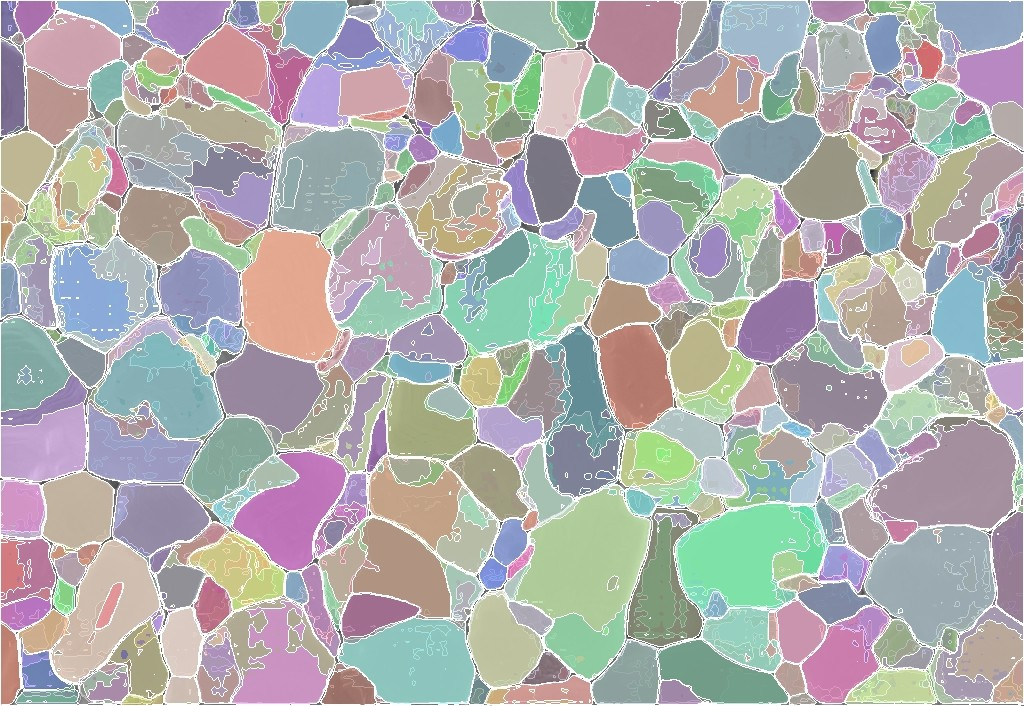
\includegraphics[width=0.92\textwidth]{Fig_sam_result.jpg}}
{
\fbox{
\begin{minipage}[c][5.0cm][c]{0.90\textwidth}
\centering
\textbf{[Figure placeholder: SAM output on SEM pinholes]}\\[4pt]
Upload comparison as \texttt{Fig\_sam\_result.jpg}.
\end{minipage}
}
}
\caption{Automatic mask generation using the Segment Anything Model (SAM). The class-agnostic model over-segments the SEM micrograph into hundreds of arbitrary mosaic patches based on surface texture and grain boundaries, entirely failing to isolate the pinhole defects. This highlights the unsuitability of generic edge-based segmentation for SEM material morphology.}
\label{fig:sam_result}
\end{figure*}

\subsection{Baseline Methods}\label{subsec:baselines}

The proposed method was compared with the following baselines:

\begin{itemize}
\item Otsu thresholding
\item CLAHE followed by Otsu thresholding
\item Canny edge detection
\item Watershed segmentation
\item Manual annotation reference
\end{itemize}

\subsection{Evaluation Metrics}\label{subsec:metrics}

Pixel-level segmentation was evaluated using precision, recall,
F1-score, and intersection over union (IoU):

\begin{equation}
Precision = \frac{TP}{TP + FP}
\label{eq:precision}
\end{equation}

\begin{equation}
Recall = \frac{TP}{TP + FN}
\label{eq:recall}
\end{equation}

\begin{equation}
F1 = \frac{2 \times Precision \times Recall}{Precision + Recall}
\label{eq:f1}
\end{equation}

\begin{equation}
IoU = \frac{TP}{TP + FP + FN}
\label{eq:iou}
\end{equation}

where $TP$, $FP$, and $FN$ represent true positives, false positives,
and false negatives, respectively.

\subsection{Ablation Study}\label{subsec:ablation}

An ablation study was conducted to examine the contribution of each
pipeline component. The full method was compared with versions without
CLAHE, without morphological refinement, and without contour-area
filtering.

%=====================================================================
% 8. RESULTS
%=====================================================================

\section{Results}\label{sec:results}

The proposed pipeline generated interpretable defect masks and
localised pinhole-like regions in SEM images. Qualitative comparison
showed that the proposed method produced more complete defect regions
than Canny edge detection and reduced over-segmentation compared
with watershed segmentation. Figure~\ref{fig:qualitative} shows
representative SEM defect detection results.

\begin{figure*}[t]
\centering
\IfFileExists{Fig2.png}
{\includegraphics[width=0.95\textwidth]{Fig2.png}}
{
\fbox{
\begin{minipage}[c][5.4cm][c]{0.92\textwidth}
\centering
Upload qualitative comparison image as \texttt{Fig2.png}.\\
Suggested panels: original SEM, manual annotation, Otsu,
CLAHE+Otsu, Canny, watershed, proposed method.
\end{minipage}
}
}
\caption{Qualitative comparison of SEM microdefect detection results
using manual annotation, classical baselines, and the proposed
materials-aware pipeline}
\label{fig:qualitative}
\end{figure*}

\subsection{Quantitative Segmentation Performance}
\label{subsec:quantitative}

\begin{table}[h]
\caption{Segmentation performance compared with manual annotation}
\label{tab:segmentation_metrics}
\begin{tabular}{@{}lcccc@{}}
\toprule
Method & Precision & Recall & F1-score & IoU \\
\midrule
Otsu thresholding          & -- & -- & -- & -- \\
CLAHE + Otsu               & -- & -- & -- & -- \\
Canny edge detection       & -- & -- & -- & -- \\
Watershed segmentation     & -- & -- & -- & -- \\
Proposed method            & -- & -- & -- & -- \\
\botrule
\end{tabular}
\end{table}

\subsection{Defect Quantification Results}
\label{subsec:defect_quantification_results}

\begin{table}[h]
\caption{Material-relevant defect descriptors extracted from SEM images}
\label{tab:defect_descriptors}
\begin{tabular}{@{}lccccc@{}}
\toprule
Sample & Defect count & Total area (px) & Mean diameter (nm) & Defect-area (\%) \\
\midrule
Sample 1 & -- & -- & -- & -- \\
Sample 2 & -- & -- & -- & -- \\
Sample 3 & -- & -- & -- & -- \\
Sample 4 & -- & -- & -- & -- \\
\botrule
\end{tabular}
\end{table}

Table~\ref{tab:defect_descriptors} shows the type of morphology
descriptors produced by the proposed pipeline. A mean defect diameter
in the range of $\sim$100--200~nm would be consistent with the
nanovoid dimensions reported by Chang et al.\ \cite{chang2026} for
similar perovskite film systems, providing a materials-grounded
interpretation of the pipeline output.

\subsection{Deep-Learning Defect Detection Results}
\label{subsec:yolo_results}

To benchmark the classical pipeline against a data-driven approach,
six YOLO models were trained on the 4{,}701-patch dataset using
the five-class annotation scheme described in
Section~\ref{subsec:sem_dataset}. Models from both the YOLOv8 and
YOLO11 families were evaluated, spanning small (s), medium (m), and
large (l) backbone configurations. All models were trained for
50~epochs at 224$\times$224~pixel resolution on an NVIDIA RTX~3050~Ti
(4~GB VRAM) GPU using Ultralytics 8.0 \cite{ultralytics2023}.

Table~\ref{tab:yolo_results} reports the precision, recall,
F1-score, mAP50, mAP50-95, and training time for each model.

\begin{table*}[t]
\caption{YOLO model comparison on the 4{,}701-patch perovskite SEM dataset
(50~epochs, 224$\times$224~px, NVIDIA RTX~3050~Ti 4~GB VRAM)}
\label{tab:yolo_results}
\begin{tabular}{@{}lcccccc@{}}
\toprule
Model & Precision & Recall & F1-score & mAP50 & mAP50-95 & Train time \\
\midrule
YOLOv8s  & 0.455 & 0.425 & 0.440 & 0.378 & 0.163 & 27.7 min \\
YOLOv8m  & 0.398 & 0.430 & 0.413 & 0.353 & 0.154 & 39.1 min \\
YOLOv8l  & 0.304 & 0.308 & 0.306 & 0.237 & 0.089 & 70.3 min \\
YOLO11s  & 0.433 & 0.458 & 0.445 & 0.396 & 0.173 & 37.3 min \\
\textbf{YOLO11m} & \textbf{0.449} & \textbf{0.482} & \textbf{0.465} & \textbf{0.422} & \textbf{0.191} & 68.5 min \\
YOLO11l  & 0.405 & 0.432 & 0.418 & 0.353 & 0.160 & 176.8 min \\
\botrule
\end{tabular}
\end{table*}

YOLO11m achieved the highest overall performance across all metrics:
mAP50 of 0.422, mAP50-95 of 0.191, precision of 0.449, recall of
0.482, and F1-score of 0.465. Compared to the smaller YOLO11s model,
YOLO11m improved mAP50 by 2.6 percentage points and mAP50-95 by
1.8 percentage points while remaining within the 4~GB VRAM budget.
The larger YOLO11l model did not show further gains, suggesting that
the current dataset size (4{,}701 patches, 440 base images) is the
primary bottleneck rather than model capacity.

The moderate mAP50-95 values across all models (0.089--0.191) reflect
the inherent difficulty of detecting nanoscale microdefects in SEM
images. Perovskite pinholes and voids appear as small, weakly
contrasted dark regions at 224$\times$224~pixel resolution, making
high-precision bounding-box localisation at strict IoU thresholds
challenging. These results are consistent with the known difficulty
of SEM defect detection at nanoscale resolution and highlight the
current dataset size as the main constraint on model performance.
The trained YOLO11m weights are available at the repository listed
in the Code Availability section.

\begin{figure*}[t]
\centering
\begin{minipage}{0.32\textwidth}
\centering

\includegraphics[width=\linewidth]{model_map5095_comparison.png}
\end{minipage}\hfill
\begin{minipage}{0.32\textwidth}
\centering

\includegraphics[width=\linewidth]{precision_recall_scatter.png}
\end{minipage}\hfill
\begin{minipage}{0.32\textwidth}
\centering

\includegraphics[width=\linewidth]{training_time.png}
\end{minipage}
\caption{Performance evaluation of the trained YOLO models. From left to right: Comparison of mAP50-95 scores across models showing YOLO11m's superior performance; precision-recall trade-off distribution; and training time requirements for 50 epochs.}
\label{fig:yolo_charts}
\end{figure*}

\subsection{Ablation Results}\label{subsec:ablation_results}

\begin{table}[h]
\caption{Ablation analysis of the proposed SEM defect quantification pipeline}
\label{tab:ablation}
\begin{tabular}{@{}lcccc@{}}
\toprule
Pipeline variant & Precision & Recall & F1-score & IoU \\
\midrule
Without CLAHE              & -- & -- & -- & -- \\
Without morphology         & -- & -- & -- & -- \\
Without contour filtering  & -- & -- & -- & -- \\
Full proposed pipeline     & -- & -- & -- & -- \\
\botrule
\end{tabular}
\end{table}

%=====================================================================
% 9. DISCUSSION
%=====================================================================

\section{Discussion}\label{sec:discussion}

The results suggest that automated SEM morphology quantification can
support materials characterisation of perovskite photovoltaic films.
The proposed method is not limited to visual enhancement; it produces
measurable descriptors that can be linked to film coverage, defect
density, and potential device-quality issues.

\subsection{Physical Interpretation of Detected Defects}

The dark regions detected by the proposed pipeline correspond to
pinhole-like and void-like morphological features. Based on recent
experimental literature, these features carry the following physical
significance. Voids of the size range targeted by the pipeline
($\sim$100--200~nm equivalent diameter) are consistent with those
reported by Chang et al.\ \cite{chang2026} in 1.67~eV wide-bandgap
perovskite films. These voids were experimentally linked to increased
trap-state density ($2.62 \times 10^{16}$~cm$^{-3}$) and reduced fill
factor. A pipeline that can automatically detect and measure such
features provides a quantitative route to assess whether a given
fabrication condition is likely to produce trap-rich or trap-lean
film morphology.

The defect-area percentage (Equation~\ref{eq:defect_area}) can be
interpreted as a proxy for the fraction of the absorber area that is
morphologically compromised. Higher defect-area percentage may
correspond to greater non-radiative recombination losses, reduced
effective absorber coverage, and increased probability of shunting
pathways. In flexible and fiber-related devices, spatial gradients in
defect-area percentage along the device geometry may indicate local
coating non-uniformities caused by substrate curvature or tension.

\subsection{Comparison with Baseline Methods}

CLAHE improved the visibility of weakly contrasted pinhole-like
regions, while dynamic thresholding reduced dependence on a single
manually chosen threshold. Morphological refinement improved the
continuity of defect masks. Contour-based filtering reduced false
positives by excluding regions that were too small or geometrically
inconsistent with material defects.

Compared with Otsu thresholding, the proposed approach provides more
direct control over defect sensitivity through the parameter $k$.
Compared with Canny edge detection, it provides filled defect regions
rather than boundary-only maps, enabling area-based quantification.
Compared with watershed segmentation, it reduces over-segmentation
in noisy SEM textures.

\subsection{Connection to Manufacturing-Scale Quality Control}

The transition from laboratory-scale to manufacturing-scale perovskite
photovoltaics requires rapid, reproducible feedback between film
deposition and morphology quality. As demonstrated in recent work on
large-area triple-junction devices \cite{zheng2025}, SEM imaging is
used to confirm that performance benchmarks are maintained when
scaling from 1~cm$^2$ to 16~cm$^2$ device areas. Automated morphology
quantification pipelines of the type proposed here are a necessary
step toward making this morphology feedback loop scalable and
objective.

Future work should validate the correlation between pipeline-derived
defect descriptors and device performance parameters such as fill
factor, open-circuit voltage, and stability---following the
experimental framework used by Chang et al.\ \cite{chang2026}, who
showed that a 14.8\% reduction in trap-state density corresponds to
measurable improvements in V$_{oc}$, FF, and PCE.

\subsection{Limitations}

The method may still classify naturally dark texture regions as
defects when they resemble pinholes. Very small defects below the
minimum area threshold may be missed. The method also depends on
image quality, magnification, and SEM acquisition settings. The
proposed pipeline should therefore be viewed as a reproducible
screening and quantification tool rather than a complete replacement
for expert materials interpretation.

%=====================================================================
% 10. ENERGY-DEVICE AND MANUFACTURING RELEVANCE
%=====================================================================

\section{Energy-Device and Manufacturing Relevance}
\label{sec:energy_relevance}

Scalable perovskite photovoltaic manufacturing requires rapid feedback
between material processing and device-quality assessment. The
importance of this feedback loop is evident from recent high-performance
demonstrations: Chang et al.\ \cite{chang2026} showed that optimising
hole-transport layer morphology to eliminate nanovoids improved the
certified efficiency of 1.67~eV wide-bandgap perovskite cells from
21.92\% to 23.42\%, with the fill factor increasing to 86.8\%. This
level of improvement, achieved through a morphological change
detectable in SEM images, demonstrates the direct manufacturing value
of SEM-based defect quantification.

At the system level, morphological quality of individual subcell
films has been shown to be a key factor in achieving high efficiency
in tandem \cite{chang2026} and triple-junction \cite{zheng2025}
architectures. In both types of devices, SEM imaging was used to
confirm the absence of voids and delamination before performance
testing, indicating that morphological verification is a standard
quality gate.

For fiber-related and flexible perovskite photovoltaic devices, the
proposed method can support quality assessment along curved surfaces
or mechanically deformable substrates. Defect descriptors such as
defect density and defect-area percentage may be used to identify
coating non-uniformity, local film failure, or morphology degradation
after bending tests. In future work, these descriptors should be
correlated with photovoltaic parameters such as open-circuit voltage,
short-circuit current density, fill factor, power conversion
efficiency, and stability retention.

%=====================================================================
% 11. LIMITATIONS AND FUTURE WORK
%=====================================================================

\section{Limitations and Future Work}\label{sec:limitations}

This study has several limitations. First, the method depends on SEM
image quality and may require parameter adjustment for different
magnifications or imaging conditions. Second, the current pipeline
is designed mainly for dark pinhole-like and void-like defects; other
defect types such as bright particles, cracks, or delamination
regions may require additional features. Third, the method should be
validated on larger datasets containing different perovskite
compositions, coating methods, flexible substrates, and fiber-shaped
device geometries. Fourth, future work should correlate extracted
defect descriptors with photovoltaic performance and stability data,
following the experimental framework established by Chang et al.\
\cite{chang2026}.

Future extensions may include deep learning-assisted segmentation,
YOLO-based defect localisation, uncertainty-aware defect
classification, and integration with high-throughput fabrication
workflows. The proposed interpretable pipeline can also serve as a
pseudo-labelling or preprocessing tool for building larger annotated
SEM datasets.

%=====================================================================
% 12. CONCLUSION
%=====================================================================

\section{Conclusion}\label{sec:conclusion}

This work presented an interpretable SEM-based microdefect
quantification pipeline for perovskite photovoltaic materials, with
emphasis on fiber-related and flexible solar-cell inspection. The
proposed method combines CLAHE-based contrast enhancement, dynamic
thresholding, morphological refinement, and contour-based filtering
to detect pinhole-like and void-like defects. The target defect
size range ($\sim$100--200~nm) is consistent with nanovoids
experimentally documented in recent high-performance wide-bandgap
perovskite device studies \cite{chang2026}, where such voids were
directly linked to 14.8\% higher trap-state density and reduced
certified efficiency. By converting SEM morphology into quantitative
descriptors such as defect count, total defect area, mean defect
diameter, and defect-area percentage, the method connects image
analysis with material-quality assessment grounded in device physics.
The pipeline was designed to be lightweight, reproducible, and
suitable for early-stage green-energy material development. Future
work will focus on validating the method across larger perovskite
datasets, applying it to curved and fiber-shaped device geometries,
and correlating SEM defect descriptors with photovoltaic performance
and mechanical stability.

%=====================================================================
% BACK MATTER
%=====================================================================

\backmatter

\bmhead{Supplementary information}
No supplementary information is available for this manuscript.

\bmhead{Acknowledgements}
The author acknowledges the institutional and laboratory support
received during this work.

% TODO: Replace with exact acknowledgement names and departments.

\section*{Declarations}

\bmhead{Funding}
No funding was received to assist with the preparation of this
manuscript.

\bmhead{Competing interests}
The author declares that there are no competing interests relevant to
the content of this article.

\bmhead{Ethics approval and consent to participate}
Not applicable.

\bmhead{Consent for publication}
Not applicable.

\bmhead{Data availability}
The datasets generated and/or analysed during the current study are
available from the corresponding author on reasonable request.

\bmhead{Materials availability}
Not applicable.

\bmhead{Code availability}
The source code used in this study is available at:
\url{https://github.com/Sahilsonii/microdefectcv}

\bmhead{Author contribution}
Sahil Soni contributed to conceptualization, methodology, software
implementation, experiments, analysis, visualization, and manuscript
preparation. The author reviewed and approved the final manuscript.

\bmhead{Use of AI-based tools}
AI-based tools were used only for language refinement, structural
organisation, and LaTeX formatting assistance. The author verified
the technical content, experimental results, references, and final
manuscript.

%=====================================================================
% APPENDIX
%=====================================================================

\begin{appendices}

\section{Additional Parameter Settings}\label{sec:appendix_parameters}

\begin{table}[h]
\caption{Extended parameter settings for reproducibility}
\label{tab:appendix_parameters}
\begin{tabular}{@{}lll@{}}
\toprule
Parameter & Value & Description \\
\midrule
CLAHE clip limit       & 3.0           & Controls contrast enhancement strength \\
CLAHE tile grid size   & $8\times8$    & Defines local histogram region \\
Gaussian blur $\sigma$ & 1.0           & Pre-CLAHE noise smoothing \\
Dark percentile        & 12.0          & Primary dark-region threshold \\
Strict dark percentile & 6.0           & Fallback threshold \\
Max fill ratio         & 0.08          & Over-segmentation guard \\
Min area (dark)        & 15~px         & Removes isolated noise \\
Min area (bright)      & 3~px          & Bright-particle sensitivity \\
Min circularity (dark) & 0.30          & Pinhole shape constraint \\
Min solidity           & 0.40          & Compact region filter \\
NMS IoU threshold      & 0.40          & Overlap suppression \\
Confidence threshold   & 0.30          & Minimum detection confidence \\
Max aspect ratio       & 5.0           & Excludes elongated artefacts \\
\botrule
\end{tabular}
\end{table}

\end{appendices}

%=====================================================================
% REFERENCES
%=====================================================================

\begin{thebibliography}{99}

\bibitem{kojima2009}
Kojima A, Teshima K, Shirai Y, Miyasaka T.
Organometal halide perovskites as visible-light sensitizers for
photovoltaic cells.
J Am Chem Soc. 2009;131:6050--6051.
\url{https://doi.org/10.1021/ja809598r}

\bibitem{snaith2013}
Snaith HJ.
Perovskites: the emergence of a new era for low-cost, high-efficiency
solar cells.
J Phys Chem Lett. 2013;4:3623--3630.
\url{https://doi.org/10.1021/jz4020162}

\bibitem{green2014}
Green MA, Ho-Baillie A, Snaith HJ.
The emergence of perovskite solar cells.
Nat Photonics. 2014;8:506--514.
\url{https://doi.org/10.1038/nphoton.2014.134}

\bibitem{park2015}
Park NG.
Perovskite solar cells: an emerging photovoltaic technology.
Mater Today. 2015;18:65--72.
\url{https://doi.org/10.1016/j.mattod.2014.07.007}

\bibitem{green2025}
Green MA, Dunlop ED, Yoshita M, Kopidakis N, Bothe K, et al.
Solar cell efficiency tables (version~66).
Prog Photovolt Res Appl. 2025;33:795--810.
\url{https://doi.org/10.1002/pip.3919}

\bibitem{chang2026}
Chang L-C, Duong T, Ahmad V, Zhan H, Bui AD, et al.
High-efficiency perovskite/silicon tandem solar cells based on
wide-bandgap perovskite solar cells with unprecedented fill factor.
Nano-Micro Lett. 2026;18:122.
\url{https://doi.org/10.1007/s40820-025-01959-y}

\bibitem{zheng2025}
Zheng J, Wang G, Duan L, Duan W, Jiang Y, et al.
Tailoring nanoscale interfaces for perovskite--perovskite--silicon
triple-junction solar cells.
Nat Nanotechnol. 2025;20:1648--1655.
\url{https://doi.org/10.1038/s41565-025-02015-x}

\bibitem{balilonda2019}
Balilonda A, Li Q, Zhu M.
Perovskite solar fibers: current status, issues and challenges.
Adv Fiber Mater. 2019;1:101--125.
\url{https://doi.org/10.1007/s42765-019-00011-0}

\bibitem{hu2016}
Hu H, Yan K, Peng M, Yu X, Chen S, Chen B, et al.
Fiber-shaped perovskite solar cells with 5.3\% efficiency.
J Mater Chem A. 2016;4:3901--3906.
\url{https://doi.org/10.1039/C5TA10slat}

\bibitem{qiu2016}
Qiu L, He S, Yang J, Deng J, Peng H.
Fiber-shaped perovskite solar cells with high power conversion efficiency.
Small. 2016;12:2419--2424.
\url{https://doi.org/10.1002/smll.201600104}

\bibitem{diGiacomo2016}
Di Giacomo F, Fakharuddin A, Jose R, Brown TM.
Progress, challenges and perspectives in flexible perovskite solar cells.
Energy Environ Sci. 2016;9:3007--3035.
\url{https://doi.org/10.1039/C6EE01137C}

\bibitem{hu2023}
Hu H, Ritzer DB, Diercks A, Li Y, Singh R, et al.
Void-free buried interface for scalable processing of p-i-n-based
FAPbI\textsubscript{3} perovskite solar modules.
Joule. 2023;7:1574--1592.
\url{https://doi.org/10.1016/j.joule.2023.05.017}

\bibitem{chen2021}
Chen S, Dai X, Xu S, Jiao H, Zhao L, Huang J.
Stabilizing perovskite--substrate interfaces for high-performance
perovskite modules.
Science. 2021;373:902--907.
\url{https://doi.org/10.1126/science.abi6323}

\bibitem{alashouri2020}
Al-Ashouri A, K\"{o}hnen E, Li B, Magomedov A, Hempel H, et al.
Monolithic perovskite/silicon tandem solar cell with $>$29\% efficiency
by enhanced hole extraction.
Science. 2020;370:1300--1309.
\url{https://doi.org/10.1126/science.abd4016}

\bibitem{otsu1979}
Otsu N.
A threshold selection method from gray-level histograms.
IEEE Trans Syst Man Cybern. 1979;9:62--66.
\url{https://doi.org/10.1109/TSMC.1979.4310076}

\bibitem{canny1986}
Canny J.
A computational approach to edge detection.
IEEE Trans Pattern Anal Mach Intell. 1986;PAMI-8:679--698.
\url{https://doi.org/10.1109/TPAMI.1986.4767851}

\bibitem{vincent1991}
Vincent L, Soille P.
Watersheds in digital spaces: an efficient algorithm based on
immersion simulations.
IEEE Trans Pattern Anal Mach Intell. 1991;13:583--598.
\url{https://doi.org/10.1109/34.87344}

\bibitem{zuiderveld1994}
Zuiderveld K.
Contrast limited adaptive histogram equalization.
In: Heckbert PS, editor. Graphics Gems IV.
San Diego: Academic Press; 1994. p. 474--485.
\url{https://doi.org/10.1016/B978-0-12-336156-1.50061-6}

\bibitem{ronneberger2015}
Ronneberger O, Fischer P, Brox T.
U-Net: convolutional networks for biomedical image segmentation.
In: Medical Image Computing and Computer-Assisted Intervention --
MICCAI 2015.
Cham: Springer; 2015. p. 234--241.
\url{https://doi.org/10.1007/978-3-319-24574-4_28}

\bibitem{redmon2016}
Redmon J, Divvala S, Girshick R, Farhadi A.
You only look once: unified, real-time object detection.
In: Proceedings of the IEEE Conference on Computer Vision and
Pattern Recognition. 2016. p. 779--788.
\url{https://doi.org/10.1109/CVPR.2016.91}

\bibitem{ultralytics2023}
Jocher G, Chaurasia A, Qiu J.
Ultralytics YOLO. Version 8.0.0.
2023. \url{https://github.com/ultralytics/ultralytics}

\bibitem{autodistill2023}
Roboflow Inc.
AutoDistill: Label datasets with foundation models.
Version 0.1.
2023. \url{https://github.com/autodistill/autodistill}

\bibitem{liu2023groundingdino}
Liu S, Zeng Z, Ren T, Li F, Zhang H, Yang J, et al.
Grounding DINO: Marrying DINO with grounded pre-training for
open-set object detection.
arXiv preprint. 2023.
\url{https://doi.org/10.48550/arXiv.2303.05499}

\bibitem{kirillov2023sam}
Kirillov A, Mintun E, Ravi N, Mao H, Rolland C, Gustafson L, et al.
Segment anything.
In: Proceedings of the IEEE/CVF International Conference on Computer
Vision (ICCV). 2023. p. 4015--4026.
\url{https://doi.org/10.1109/ICCV51070.2023.00371}

\bibitem{ref23}
% TODO: Replace with the correct reference for the FAPbI3 one-pot
% synthesis and 2D/3D surface treatment protocol (GreatCell Solar materials).
Author A, Author B.
Title of fabrication protocol reference.
Journal. Year;Volume:Pages.

\end{thebibliography}

\end{document}